\subsection{Stitching}
The stitching was performed with two different blending functions. The result of stitching image one and two with a linear transision is shown in figure \ref{fig:results:stitching:linear} and the corresponding one using a sigmoid function is shown in figure \ref{fig:results:stitching:sigmoid}. A stitching performed when using two cameras in a home made set-up is found in figure \ref{fig:results:stitching:homemade}.

\begin{figure}[H]
  \centering
  \includegraphics[width = 0.9\columnwidth]{../results/stitch_linear.jpg}
  \caption{Stitching done using a linear transition.}
  \label{fig:results:stitching:linear}
\end{figure}

\begin{figure}[H]
  \centering
  \includegraphics[width = 0.9\columnwidth]{../results/stitch_sigmoid.jpg}
  \caption{Stitching done using a sigmoid transition.}
  \label{fig:results:stitching:sigmoid}
\end{figure}

\begin{figure*}
	\centering
	\begin{subfigure}[t]{0.3\textwidth}
		\centering
		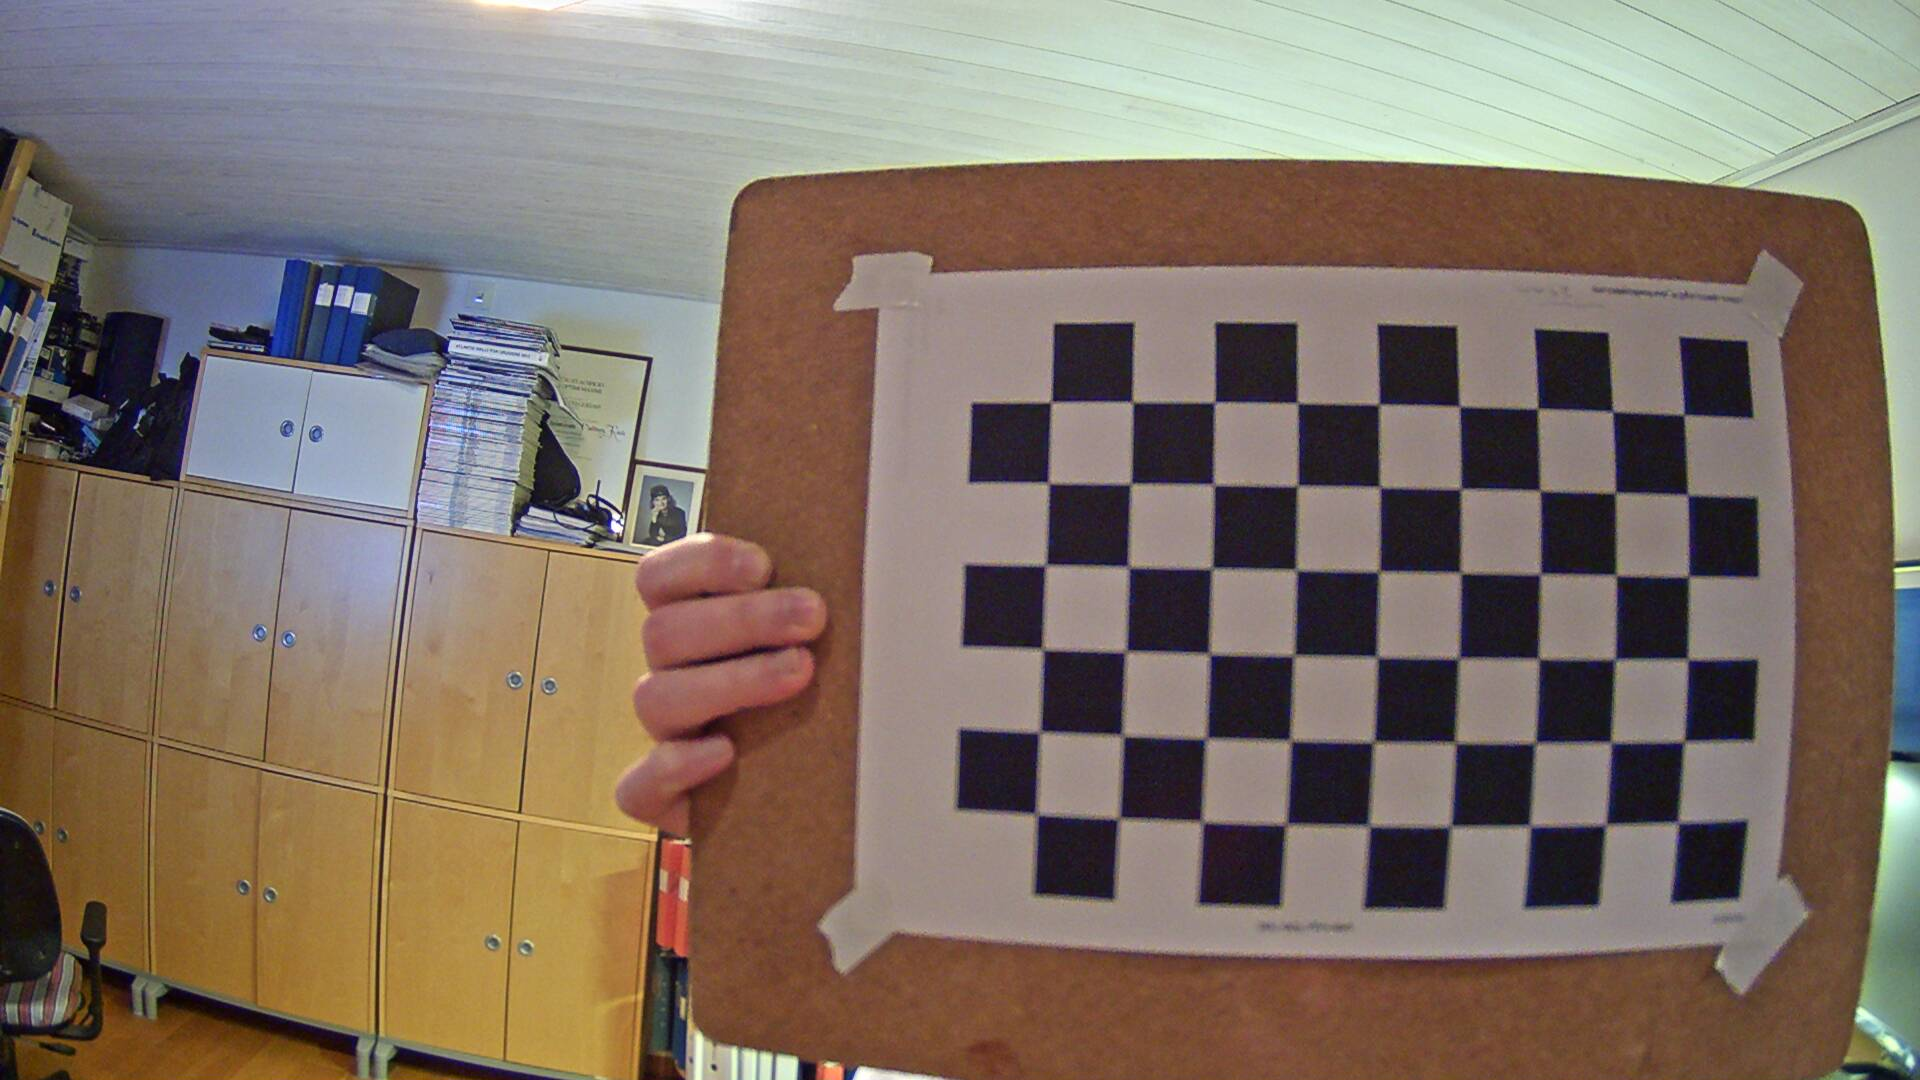
\includegraphics[width=\textwidth]{../data/homography/camera_1.jpg}
		\caption{input 1}
	\end{subfigure}
	\begin{subfigure}[t]{0.3\textwidth}
		\centering
		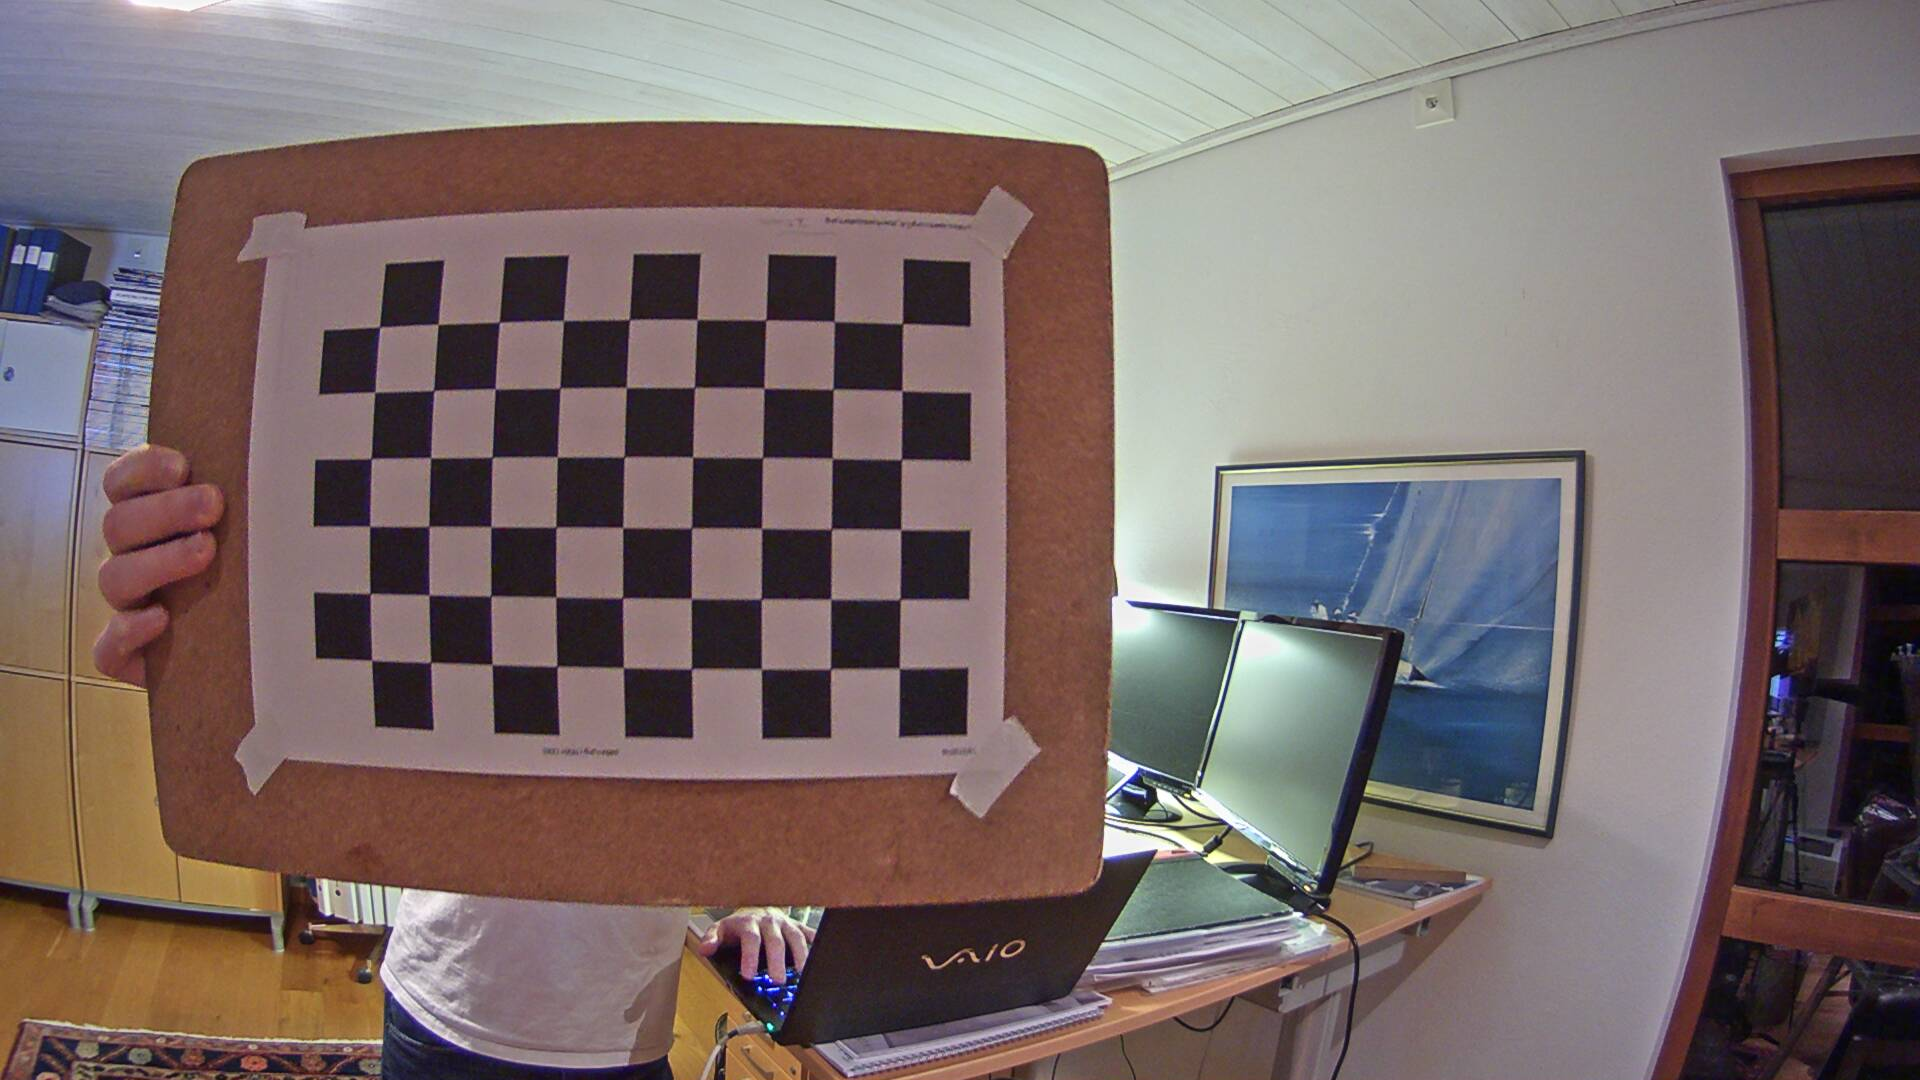
\includegraphics[width=\textwidth]{../data/homography/camera_2.jpg}
		\caption{input 2}
	\end{subfigure}
		\begin{subfigure}[t]{0.3\textwidth}
		\centering
                \includegraphics[width = \textwidth]{../results/home_made_stitch.jpg}
		\caption{output}
	\end{subfigure}
        \caption{Stitching done with home made set-up.}
	\label{fig:results:stitching:homemade}
\end{figure*}
